%%%%%%%%%%%%%%%%%%%%%%%%%%%%%%%%%%%%%%%%%%%%%%%%%%%%%%%%%%%%%%%%%%%%%%%%%%%%
% Supporting Information for AGU Journal Submission
% Uses same document class as main manuscript for consistent formatting
%%%%%%%%%%%%%%%%%%%%%%%%%%%%%%%%%%%%%%%%%%%%%%%%%%%%%%%%%%%%%%%%%%%%%%%%%%%%

\documentclass{agujournal2019}
\usepackage{url}
\usepackage{booktabs}
\usepackage{siunitx}
\sisetup{separate-uncertainty=true}

% Graphics handling
\usepackage{graphicx}
\setkeys{Gin}{draft=false}

% Cross-referencing (hyperref required for proper .aux generation)
%\usepackage{hyperref}

% Journal name (same as main manuscript)
\journalname{JGR: Biogeosciences}

\begin{document}

\renewcommand{\thefigure}{S\arabic{figure}}
\renewcommand{\thetable}{S\arabic{table}}

%% Supporting Information Title
\title{Supporting Information for ``Reversible Regime Change: Climate-driven phytoplankton community shifts in the Cariaco Basin, Venezuela''}

\authors{Benjamin Post\affil{1,2}, Esteban Acevedo-Trejos\affil{1,3}, Subhendu Chakraborty\affil{1}, Andrew D. Barton\affil{4}, Agostino Merico\affil{1,2,5}}

\affiliation{1}{Leibniz Centre for Tropical Marine Research (ZMT), Bremen, Germany}
\affiliation{2}{School of Science, Constructor University, Bremen, Germany}
\affiliation{3}{Earth Surface Process Modelling, GFZ German Research Centre for Geosciences, Potsdam, Germany}
\affiliation{4}{Scripps Institution of Oceanography and Department of Ecology, Behavior and Evolution, University of California San Diego, La Jolla, CA, United States}
\affiliation{5}{Faculty of Biology and Chemistry (FB2), University of Bremen, Germany}

\correspondingauthor{Benjamin Post}{benjaminpost@aoop.de}

%% No abstract for SI
\begin{keypoints}
\item Temporal clustering of phytoplankton communities is robust across different distance metrics and linkage methods
\item Interannual variability explains five times more community variance than seasonal effects
\item Seasonal gradient forest analyses support main findings while revealing season-specific environmental drivers
\end{keypoints}

\section*{Contents of this file}
\begin{enumerate}
\item Figure S1: Comparison of hierarchical clustering methods for annual community data
\item Figure S2: NMDS ordination of monthly communities colored by season
\item Figure S3: Gradient forest predictor importance by oceanographic season
\item Table S1: PERMANOVA comparing interannual cluster vs.\ seasonal effects
\item Table S2: Optimal lag selection for environmental predictor variables
\end{enumerate}

\newpage
\section{Annual Clustering Supplemental Information}

\begin{figure}[ht]
\centering
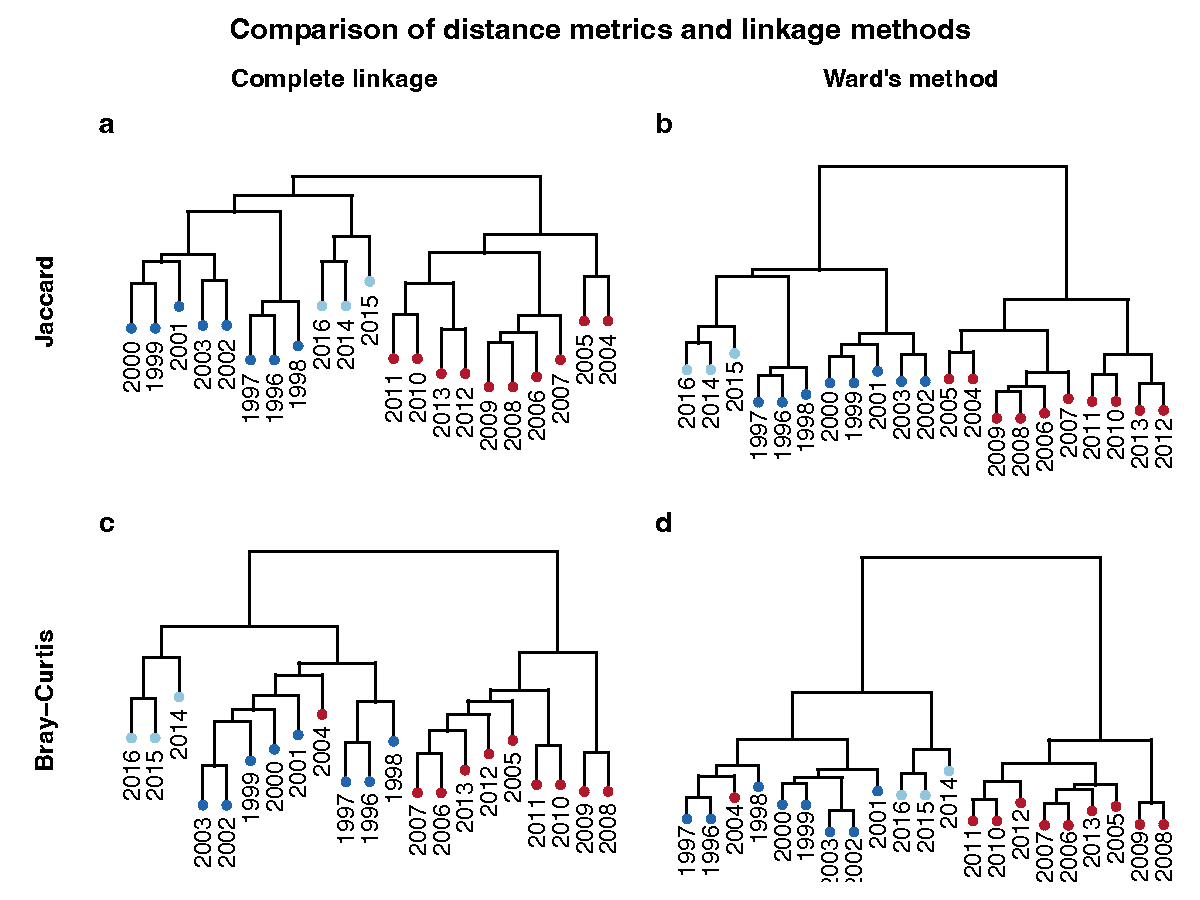
\includegraphics[width=\textwidth]{Supplemental_ClusteringComparison.pdf}
\caption{Comparison of hierarchical clustering methods applied to annually aggregated phytoplankton community data (1996--2016). Four combinations of distance metrics and linkage methods are shown: (a) Jaccard dissimilarity with complete linkage, (b) Jaccard dissimilarity with Ward's method, (c) Bray-Curtis dissimilarity with complete linkage, and (d) Bray-Curtis dissimilarity with Ward's method. Jaccard dissimilarity was calculated on presence/absence data, while Bray-Curtis dissimilarity was calculated on cube-root transformed mean annual abundances, calculated from 0--100~m depth-integrated cell counts at the genus level. Colors indicate cluster assignments based on the reference clustering (from the complete linkage clustering based on the Jaccard distance): dark blue = Early Cluster~1 (1996--2003), dark red = Cluster~2 (2004--2013), light blue = Late Cluster~1 (2014--2016). All four methods recovered nearly identical cluster assignments, with only 2004 assigned differently by Ward's method, demonstrating that the identified temporal pattern is robust to methodological choices.}
\label{fig:sup:annual_clust_comp}
\end{figure}

\clearpage
\section{Seasonal Effect Supplemental Information}

\begin{figure}[ht]
\centering
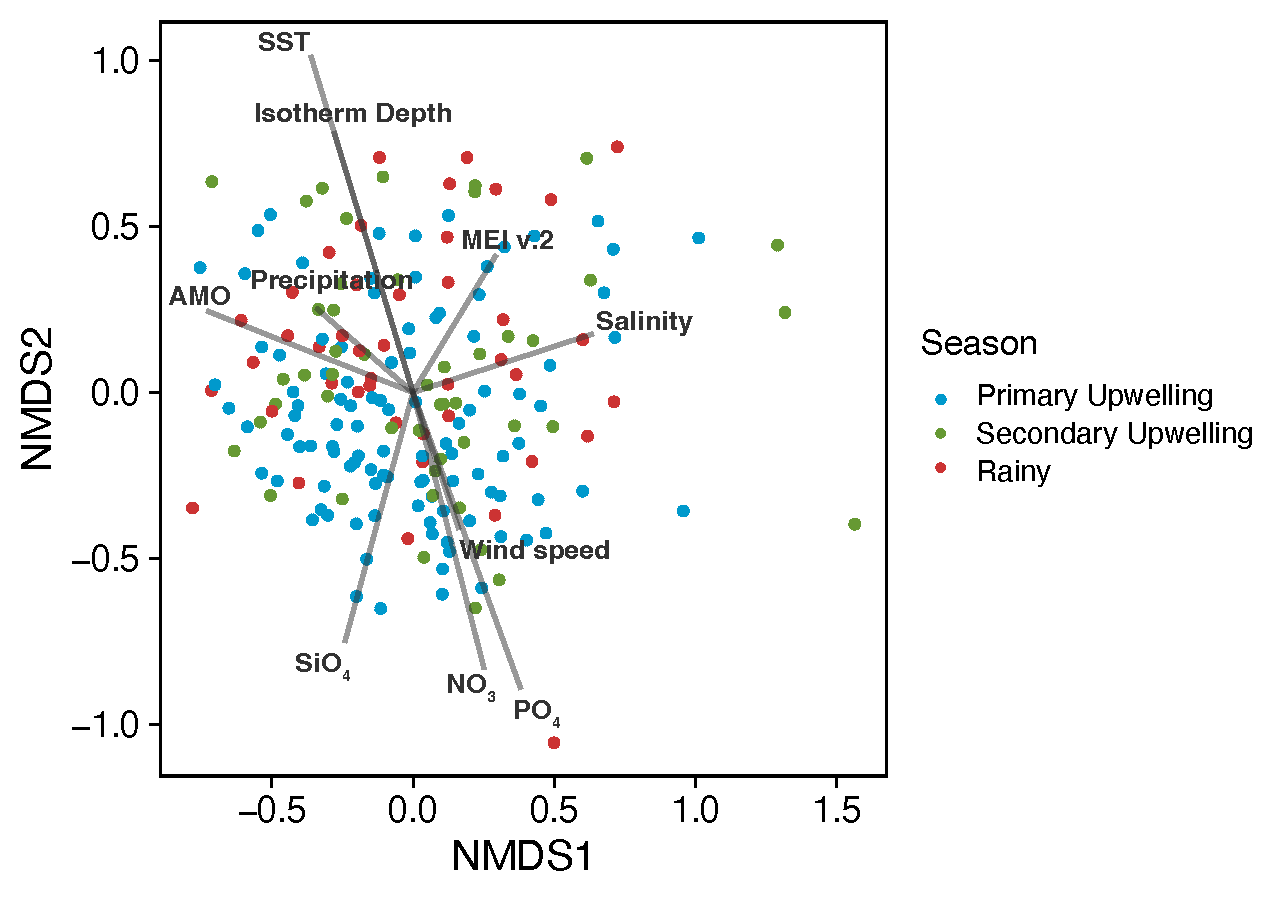
\includegraphics[width=0.75\textwidth]{FigureSX_seasonalNMDS_v1.pdf}
\caption{NMDS plot of monthly phytoplankton community data (genus-level cell counts, cube-root transformed) with points colored by season. Stress: 0.263, 2 dimensions, converging solution. Vectors show how environmental variables co-vary with the community data. Vector length indicates the strength of the relationship. No clear separation is visible among seasonal groups (Upwelling: December--May, Secondary Upwelling: June--August, Rainy: September--November), consistent with PERMANOVA results showing that season explains only 3.5\% of community variance compared to 17.9\% for interannual clusters (Table~\ref{tab:sup:permanova_season_cluster}).}
\label{fig:sup:nmds_season}
\end{figure}

\begin{table}[ht]
\centering
\caption{Permutational multivariate analysis of variance (PERMANOVA) testing the effects of interannual clusters and season on phytoplankton community composition. Community data (genus-level cell counts) were cube-root transformed prior to analysis. Bray-Curtis dissimilarity was used as the distance metric, with 999 permutations. Observations from 1995 and 2017 were excluded due to missing cluster assignments ($n = 193$). Results shown are for cluster entered first. Reversing term order yielded identical $R^{2}$ values (cluster: 17.9\%, season: 3.5\%), indicating minimal collinearity between factors.}
\label{tab:sup:permanova_season_cluster}
\begin{tabular}{l r r r r l}
\hline
Factor & df & Sum of Squares & $R^{2}$ (\%) & $F$ & $p$-value \\
\hline
Cluster & 2 & 8.772 & 17.9 & 21.4 & 0.001 \\
Season & 2 & 1.713 & 3.5 & 4.2 & 0.001 \\
Residual & 188 & 38.525 & 78.6 & --- & --- \\
Total & 192 & 49.010 & 100.0 & --- & --- \\
\hline
\end{tabular}
\end{table}

\clearpage

\begin{table}[ht]
\centering
\caption{Mean $R^2$ weighted importance for predictor variables across three seasons, used to select optimal time lags. Values shown as: lag in months (mean importance). Due to relatively small seasonal sample sizes and resulting stochasticity in importance estimates, the analysis was run five times per season and mean values are reported. For in-situ variables, lags of 0--3 months were tested; for atmospheric variables, 0--6 months; for climate indices, 0, 12, 24, 36, 48, and 60 months. To balance model parsimony with explanatory power, the shortest lag within 20\% of maximum importance was selected (bold), favoring more directly interpretable ecological relationships when predictive performance was similar.}
\label{tab:sup:GFlagtests_seasonal}
\small
\resizebox{\textwidth}{!}{%
\begin{tabular}{llll}
\toprule
Variable & Upwelling & Secondary Upwelling & Rainy\\
\midrule
\multicolumn{4}{l}{\textit{In-situ variables (lags 0--3 months)}}\\
\quad NO\textsubscript{3} & \textbf{0} (0.060); 1 (0.036); 2 (0.020) & \textbf{0} (0.034); 3 (0.031); 2 (0.029) & 3 (0.017); \textbf{0} (0.015); 2 (0.006)\\
\quad PO\textsubscript{4} & \textbf{0} (0.023); 1 (0.008); 2 (0.007) & 3 (0.023); \textbf{0} (0.021); 2 (0.020) & \textbf{0} (0.039); 3 (0.027); 1 (0.014)\\
\quad SiO\textsubscript{4} & \textbf{0} (0.026); 1 (0.008); 3 (0.006) & \textbf{0} (0.032); 1 (0.028); 2 (0.022) & \textbf{3} (0.043); 1 (0.033); 2 (0.032)\\
\quad SST & \textbf{0} (0.101); 3 (0.014); 1 (0.007) & \textbf{0} (0.032); 2 (0.025); 1 (0.014) & \textbf{0} (0.052); 1 (0.032); 3 (0.010)\\
\quad 21\,\textdegree C Isotherm & \textbf{0} (0.045); 1 (0.011); 2 (0.007) & \textbf{1} (0.024); 3 (0.014); 0 (0.010) & \textbf{0} (0.032); 2 (0.010); 3 (0.007)\\
\quad Salinity & \textbf{0} (0.031); 3 (0.010); 2 (0.008) & \textbf{2} (0.073); 3 (0.049); 1 (0.020) & \textbf{0} (0.022); 3 (0.010); 2 (0.010)\\
\addlinespace
\multicolumn{4}{l}{\textit{Atmospheric variables (lags 0--6 months)}}\\
\quad Wind speed & 5 (0.007); 6 (0.007); \textbf{4} (0.006) & \textbf{6} (0.027); 2 (0.010); 5 (0.006) & \textbf{0} (0.021); 5 (0.019); 2 (0.009)\\
\quad Precipitation & \textbf{1} (0.019); 0 (0.012); 2 (0.009) & \textbf{0} (0.018); 2 (0.012); 1 (0.008) & \textbf{3} (0.017); 0 (0.012); 6 (0.006)\\
\addlinespace
\multicolumn{4}{l}{\textit{Climate indices (lags 0, 12, 24, 36, 48, 60 months)}}\\
\quad AMO & 60 (0.028); \textbf{24} (0.023); 36 (0.021) & \textbf{24} (0.034); 60 (0.032); 36 (0.020) & 48 (0.028); \textbf{36} (0.025); 12 (0.013)\\
\quad MEI v.2 & \textbf{48} (0.036); 36 (0.018); 60 (0.018) & \textbf{60} (0.037); 24 (0.018); 0 (0.015) & 48 (0.027); \textbf{36} (0.024); 60 (0.020)\\
\bottomrule
\end{tabular}%
}
\end{table}

\clearpage

\begin{figure}[ht]
\centering
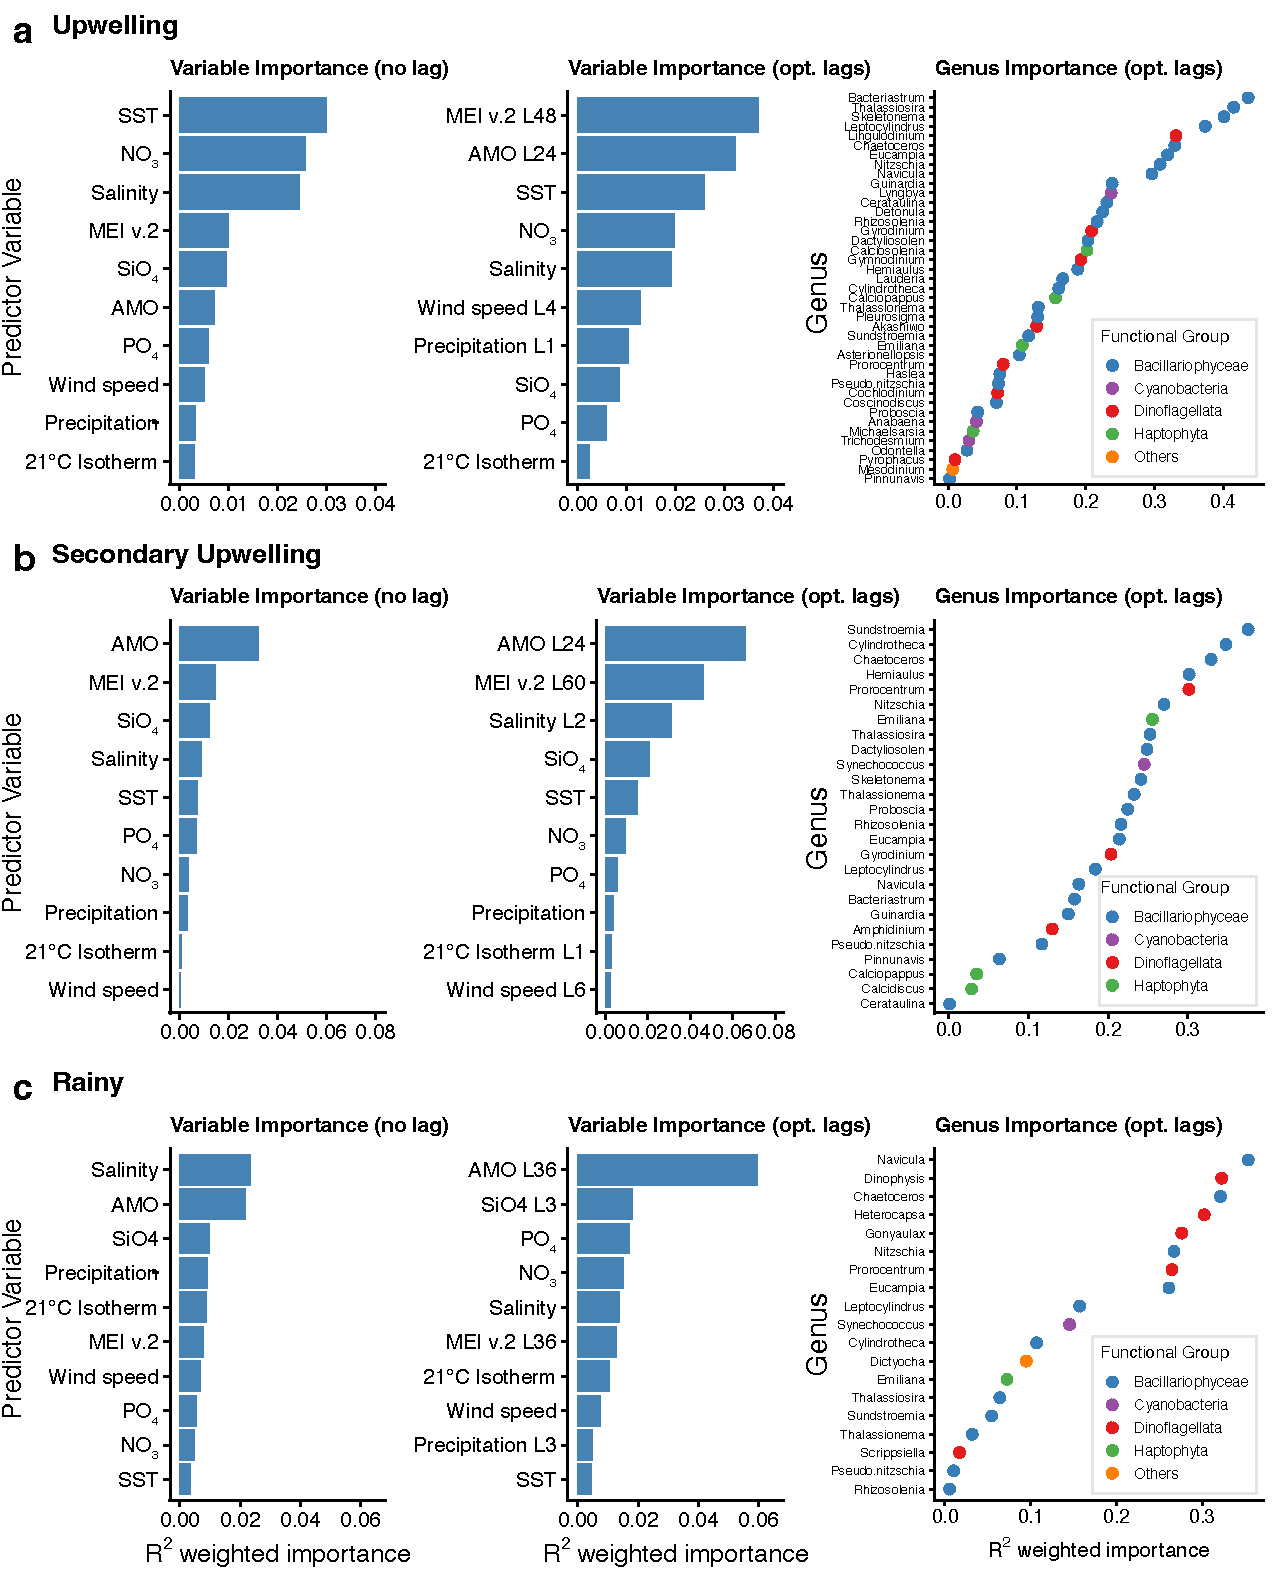
\includegraphics[width=\textwidth]{FigureS3_GF_seasonal_ALL_COMBINED.pdf}
\caption{Exploratory gradient forest analysis of monthly phytoplankton community data at genus level across three oceanographic seasons: (a) Primary Upwelling (December--May), (b) Secondary Upwelling (June--August), and (c) Rainy Season (September--November). For each season, predictor variables are ranked by $R^2$ weighted importance for models without time lags (left) and with optimal lags (center), where lag notation indicates number of months (e.g., L24 = 24-month lag). The right panels show phytoplankton genera ranked by predictive power under optimal lag conditions, colored by functional group. Slight variation occurs between runs due to the stochastic nature of random forests; general patterns are robust. The shown results are exemplary outputs from a single model run. Monthly sample sizes per season are Primary Upwelling: $n=104$ (no lag), $n=104$ (with lags); Secondary Upwelling: $n=48$ (no lag), $n=40$ (with lags); Rainy Season: $n=43$ (no lag), $n=39$ (with lags).}
\label{fig:sup:GF_seasonal}
\end{figure}

\end{document}